\documentclass[11pt]{article}
\usepackage[margin=25mm]{geometry}
\usepackage[T1]{fontenc}
\usepackage{lmodern}
\usepackage{amsmath,amssymb,booktabs,array,graphicx}
\usepackage[colorlinks=true,linkcolor=blue,citecolor=blue,urlcolor=blue]{hyperref}
\usepackage[braket,qm]{qcircuit}
\newtheorem{theorem}{Theorem}
\newtheorem{lemma}{Lemma}
\newtheorem{proposition}{Proposition}
\newenvironment{proof}[1][Proof]{\par\noindent\textit{#1.}\ }{\hfill\textit{QED}\par}
\renewcommand{\labelitemi}{$\bullet$}
\setlength{\emergencystretch}{3em}
\newcommand{\OSR}{\operatorname{OSR}}
\newcommand{\CNOT}{\mathrm{CX}}
\newcommand{\Sqi}{\mathrm{SQiSW}}
\newcommand{\A}{\mathcal A}
\newcommand{\Id}{\mathbb I}
\title{Supplement: constructions, reference data, and experiments}
\author{Gregory Morse$^{1}$ \and P\'eter Rakyta$^{2,3}$}
\date{8 November 2026}
\begin{document}\maketitle
\begin{center}\small
$^1$Department of Programming Languages and Compilers, E\"otv\"os Lor\'and University, Hungary\\
$^2$Department of Physics of Complex Systems, E\"otv\"os Lor\'and University, Hungary\\
$^3$Computational Sciences Department, HUN-REN Wigner Research Centre for Physics, Hungary
\end{center}
This supplement accompanies \emph{Controlling two-qubit involutions:
CNOT costs and symbolic invariants}. It contains the reference resource,
all measured compiler comparisons and negative results, native-column gap
audits, and implementation details. Its empirical comparisons are separate
from the interaction-count theorems in the main paper.
\tableofcontents
\section{Symbolic constructions and reference resources}
The implementation accepts exact matrices and named symbolic families.
It enumerates all distinct nontrivial cuts, factors rank-one realignments,
and peels candidate interactions in a bounded residual search. Exact
exponential-polynomial arithmetic supplies rank witnesses rather than
numerically thresholded SVDs. Native controlled, exchange, B, and SQiSW
charts supply complementary candidates. Every accepted candidate is checked
by an exact identity or a compositional certificate of proved replacements.
A failed search remains unresolved, and a search deadline is not an
impossibility argument.

The B and SQiSW charts include folded-angle and degenerate branches.
Long expressions are stored as a scalar directed acyclic program with scoped
aliases. The canonical three-SQiSW projective chart has 585 scalar bindings
and 11 physical gates. This is a machine-inspectable exact expression
program, not a short human-readable formula. Numerical evaluation compiles
the shared dependencies once and evaluates only the branches required for
a binding; the exact family verifier remains the acceptance criterion.
The numerical binding experiment in this supplement measures this implementation without
claiming that symbolic synthesis is always faster than numerical synthesis.

The grid contains 327 catalog entries crossed with 32 supplied alphabets.
There are 217 named one-qubit entries, including 192 matrices obtained from
24 Clifford representatives and eight phases; the remaining named widths
are 72 two-qubit, 14 three-qubit, three four-qubit, and one five-qubit entry.
Twenty register fixtures use specified widths. Their physical widths produce
218, 79, 26, 3, and 1 entries at widths one through five. Aliases and phase
multiples are included explicitly and are not independent families.
In literal mode, 222 entries admit zero-entangler constructions in every preset
where they are representable; zero-cost nonlocal synthesis is not inferred
from the size of the headline grid.

The Clifford reference includes finite-alphabet shortest-path proofs for
$\{H,S,T,T^\dagger\}$: a radius-seven search reaches 628 matrices, and
meet-in-the-middle splitting proves word minima for all 192 targets, with
maximum length fourteen. Continuous-alphabet circuits have no corresponding
unrestricted local-optimality claim. The result is a useful explicit phase
reference alongside established Clifford+T synthesis theory
\cite{matsumoto,kmm,giles,gilesma}. The actual gate and Clifford PDFs, their
editable LaTeX, alphabetical index, and exact expression glossaries are
included in the full review package.

\section{Evaluation}
\subsection{Coverage by width and proof scope}
The following tables classify every effective cell, including a literal
circuit reused as its projective construction. ``Fixed min.'' and ``Family
min.'' are a disjoint union of matching explicit lower-bound payloads. The
latter certifies a necessary uniform family budget, not the minimum at every
parameter specialization. ``Unproved'' means that a positive-entangler
construction lacks a matched certificate in this union. Legacy Boolean
optimality flags alone are not counted as proof payloads. Zero-entangler
constructions and obstructions appear separately.
\paragraph{Literal equality.}\begin{center}\small\begin{tabular}{lrrrrrrr}\toprule
Qubits & Cells & $E=0$ & $E>0$ & Fixed min. & Family min. & Unproved & Obstructed\\\midrule
1 & 6976 & 5210 & 0 & 0 & 0 & 0 & 1766\\
2 & 2528 & 117 & 1754 & 689 & 710 & 355 & 657\\
3 & 832 & 80 & 468 & 43 & 0 & 425 & 284\\
4 & 96 & 0 & 59 & 0 & 0 & 59 & 37\\
5 & 32 & 0 & 14 & 0 & 0 & 14 & 18\\
Total & 10464 & 5407 & 2295 & 732 & 710 & 853 & 2762\\
\bottomrule\end{tabular}\end{center}

\paragraph{Projective equality.}\begin{center}\small\begin{tabular}{lrrrrrrr}\toprule
Qubits & Cells & $E=0$ & $E>0$ & Fixed min. & Family min. & Unproved & Obstructed\\\midrule
1 & 6976 & 6915 & 0 & 0 & 0 & 0 & 61\\
2 & 2528 & 128 & 2247 & 954 & 955 & 338 & 153\\
3 & 832 & 96 & 692 & 48 & 0 & 644 & 44\\
4 & 96 & 0 & 89 & 0 & 0 & 89 & 7\\
5 & 32 & 0 & 29 & 0 & 0 & 29 & 3\\
Total & 10464 & 7139 & 3057 & 1002 & 955 & 1100 & 268\\
\bottomrule\end{tabular}\end{center}

The row ledger lists gate, alphabet, phase policy, width, interaction count,
proof scope, and every matched proof source. This resolves the earlier
inconsistency between per-result flags and separate audit totals. In the
pre-revision archive the raw positive-entangler flags were 694 literal and
423 explicitly stored projective results. Its 1,916 explicitly stored
positive-entangler projective results omitted 1,141 positive-entangler
literal circuits reused projectively. The denominator for the complete
projective grid is therefore 3,057, not 1,916. Neither the flags nor an
uncorrected sum of overlapping audits is our reported optimality total.

The obstruction breakdown is as follows.
\begin{center}\small\begin{tabular}{lrr}\toprule
Obstruction & Literal & Projective\\\midrule
determinant\_and\_clifford\_t\_field & 0 & 16\\
determinant\_group & 2601 & 0\\
discrete\_alphabet\_nonconstant\_family & 142 & 210\\
not\_a\_clifford & 13 & 38\\
outside\_clifford\_t\_number\_field & 6 & 4\\
\bottomrule\end{tabular}\end{center}

These are standard necessary conditions, used to describe feasibility.
In particular, 2,601 literal obstructions are determinant-group tests, and
all 268 projective obstructions occur in the three discrete Clifford or
Clifford+T presets. A nonconstant continuous family cannot be covered by a
countable discrete alphabet, although special parameter values can be
representable. We do not present these simple feasibility checks as new
lower-bound theorems.

\subsection{Independent compiler comparisons}
Eight fixed targets are constructed independently from library gates.
Qiskit 2.6.2, pytket 2.18.5, and BQSKit 1.2.1 receive these source words;
for targets on at most three qubits they also receive the target matrix.
The table selects the smallest verified $(E,L)$ pair over those recorded
routes. The source is never our optimized output. Qiskit uses optimization
level three and seed 219; tket uses full peephole optimization with implicit
swaps disabled; BQSKit uses level three, maximum synthesis size three, and
a 120-second process budget. All inputs are arbitrary states, ancilla-free,
with fixed output wires and all-to-all connectivity. Full-matrix projective
replay requires maximum entry error below $10^{-8}$.

Quartz and the original Java-17 QUESO implementation receive the same
independent sources in the NAM alphabet $\{H,R_z,X,\CNOT\}$. Each has a
10-second search budget and optimizes total native gate count. Quartz uses
its supplied NAM equivalence set; QUESO rules are generated with three wires
and length six. Rule files, repository revisions, the Quartz harness patch,
and output QASM are archived. Their displayed local counts use one-qubit
fusion into U3, preserving the entangling skeleton; these settings do not
constitute an exhaustive search for each tool's best possible result.
\begin{center}\small\begin{tabular}{lrrrrrr}\toprule
Gate & Qiskit & tket & BQSKit & Quartz & QUESO & Exact atlas\\\midrule
SYC & 3/8 & 3/7 & 3/4 & 4/5 & 4/5 & 3/3\\
iSWAP & 2/3 & 2/4 & 2/4 & 2/3 & 2/3 & 2/3\\
SSWAP & 3/8 & 3/7 & 3/5 & -- & 3/8 & 3/7\\
fFredkin & 5/13 & 10/15 & 4/6 & 9/10 & 13/10 & 4/6\\
CCX & 6/8 & 6/8 & 6/8 & 6/8 & 6/8 & 6/8\\
CSWAP & 7/10 & 7/8 & 7/9 & 8/8 & 8/8 & 7/10\\
C3X & 14/19 & 14/16 & 14/16 & 14/16 & 14/16 & 14/17\\
C4X & 36/41 & 36/41 & -- & 30/33 & 36/36 & 36/41\\
\bottomrule\end{tabular}\end{center}

Entries show $E/L$; ``--'' means no output passed the declared replay
threshold on the recorded route. BQSKit has one runtime error, one
120-second exhaustion, and an unverified 30-CX C4X output. Quartz's SSWAP
output has error about $6.9\times10^{-7}$ and is excluded. Every failure and
its settings remain in the raw record.

BQSKit independently matches our fFredkin count of four CNOTs and six
locals. A separate enumeration of all 27 three-edge and 81 four-edge layouts,
with three BQSKit starts per layout, also finds a four-CNOT fit in about six
seconds overall. Failed numerical three-CNOT fits are not the lower-bound
proof. The eleven older SDK entangler wins were all fFredkin in different
presets; they were not eleven distinct gate discoveries. The current data
also contain genuine losses: Quartz reaches 30 CNOTs for C4X while this
atlas entry has 36; tket and BQSKit use fewer C3X locals; BQSKit uses fewer
SSWAP locals. Consequently we claim neither compiler dominance nor that
all atlas cells attain the best known upper bound.

The older ancilla-free SDK sources use 14 CX for C3X and 36 for C4X
\cite{maslov,qiskitsynthesis}; 36 is a historical construction, not a
best-known claim. We also checked the no-helper-qubit constructions of
Huang--Palsberg \cite{hp24} and Vale et al.\ \cite{vale24}, through their
Qiskit 2.6.2 implementations. For C4X, full literal replay verifies
52/47 CX (levels zero/three) for HP24, and 36/36 for V24 and the existing
SP22 route. The archived fixed C4X source is also 36/36. These particular
routes do not beat Quartz's verified 30-CX result; asymptotic general-purpose
bounds do not establish the smallest four-control count. The bounded
literature/implementation audit is not an exhaustive best-published census.
Ordinary Fredkin has a known seven-CX word \cite{fredkinshallow}.
Toffoli's six-CX minimum
is proved \cite{toffolicnot}; the five-unrestricted-gate Fredkin result
\cite{yuying} uses a different primitive. UniversalQCompiler is the only
listed analytical package without a run here, because its licensed Wolfram
kernel was unavailable.

\subsection{Component ablations}
Six opaque two-qubit families are tested in B/U3 and SQiSW/U3: X/Y-controlled
rotations, unequal controlled SU(2) branches, a phase-gauged exchange block,
a gauged affine Cartan family, and unequal commuting exchanges. An earlier
chart-disabled experiment verifies 3/12, compared with 11/12 for the full
method. This establishes that native charts account for much of this
workload's success.

We now separately disable OSR factor construction and residual interaction
peeling, retaining the native charts, Clifford and commuting-Pauli
constructors, and posthoc identity/lower-bound checks. Both methods receive
opaque matrices and a 20-second outer deadline, with a 0.2-second residual
search budget where enabled. The additional three- and four-qubit probes
are explicitly defined independent-product circuits, not catalog names.
\begin{center}\small\begin{tabular}{llrrrrr}\toprule
Qubits & Method & Cases & Verified & Unresolved & Deadline & Errors\\\midrule
2 & Full & 12 & 11 & 0 & 1 & 0\\
2 & OSR construction off & 12 & 11 & 0 & 1 & 0\\
3 & Full & 1 & 0 & 1 & 0 & 0\\
3 & OSR construction off & 1 & 0 & 1 & 0 & 0\\
4 & Full & 1 & 0 & 1 & 0 & 0\\
4 & OSR construction off & 1 & 0 & 1 & 0 & 0\\
\bottomrule\end{tabular}\end{center}

Figure~\ref{fig:ablation} displays these results. OSR construction does not
increase the success count on the two-qubit chart workload, and neither
method resolves the wider probes within this configuration. This experiment
does not support attributing the chart successes to OSR search. OSR's role
in the mathematical lower bounds is established analytically, independently
of the ablation. The main paper accordingly attributes its mathematical results to the analytical arguments.
\begin{figure}[ht]
\centering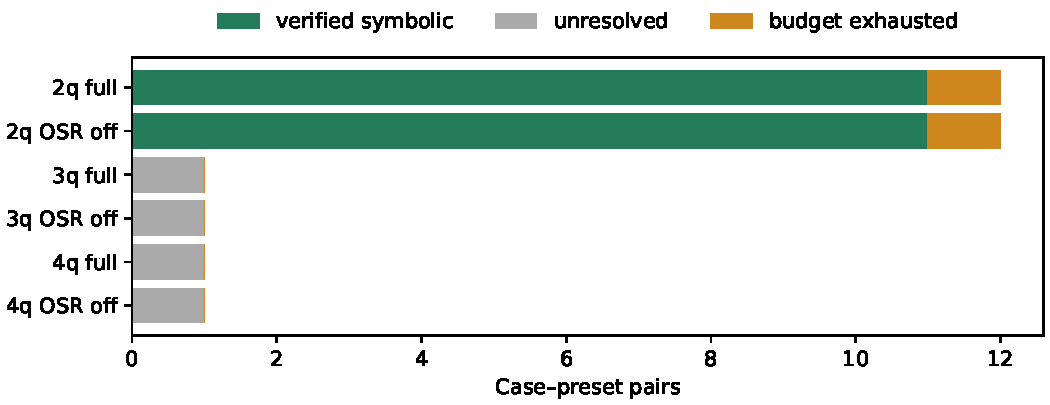
\includegraphics[width=.9\linewidth]{generated/referee_ablation.pdf}
\caption{The full constructor and the constructor with OSR factorization and
residual search disabled. The two-qubit workload is dominated by native
charts. Wider unresolved probes are retained.}\label{fig:ablation}
\end{figure}

\subsection{Parameter reuse and binding cost}
The four-qubit example composes six fSim blocks on $(0,1),(2,3),(1,2)$
repeated twice, with twelve independent parameters. A gatewise source
$R_{xx}(\theta)R_{yy}(\theta)CP(-\phi)$ is compared with a three-CX
analytical source, using the same Qiskit 2.2.3 optimization. Three-CX fSim synthesis
is established analytical knowledge, not a new resource bound.
\begin{center}\small\begin{tabular}{lrrrrr}\toprule
Route & $E$ & $L$ & Depth & Compile (ms) & 1,000 binds (ms)\\\midrule
Gatewise analytical source & 36 & 66 & 55 & 50.76 & 114.28\\
Three-CX symbolic source & 18 & 42 & 31 & 7.13 & 52.14\\
Numerical compile per binding & 18 & 40 & 25 & 7.68 & --\\
\bottomrule\end{tabular}\end{center}

The numerical row is the mean compilation time over ten independently
bound instances; all ten give $18/40/25$. It beats the symbolic circuit in
locals and depth. The weak gatewise $36/66/55$ row is retained for context
and is not evidence of improvement over the known three-CX construction.
Using that known analytical source as a compile-once control gives the same
interaction budget as the symbolic route. Qiskit already supports parameter
reuse \cite{qiskitparameter}. Cold symbolic chart synthesis took 5.63 seconds
in this run; the displayed SDK time excludes that cost. Ten complete
16-by-16 numerical replays check the composed family, whose constituent
identities are separately proved exactly.

For the larger 585-binding scalar DAG, compilation took about 1.36 seconds
and 1,000 warm evaluations about 0.97 seconds. Full two-qubit matrix replay
passed for 64 parameter assignments, including the identity, an Ising corner,
the SWAP-class corner, and 60 seeded points spanning multiple angle folds.
These are numerical regression tests of an exactly certified chart. They
show that a large symbolic program can be reused without repeated symbolic
substitution; they do not establish a speed advantage over bind-time KAK
on arbitrary workloads. Symbolic outputs are valuable when a free-parameter
identity, phase contract, or reusable expression is needed; specialization
and numerical optimization remain useful alternatives.

\subsection{A benchmark-suite peephole check}
We apply a deliberately simple atlas peephole pass to every existing
IBMEagle and QASMBenchmarks QASM source with two to eight declared qubits
and fewer than 500 semicolons, yielding eight circuits. Numerical
fingerprints propose contiguous windows of at most eight operations on two
wires; exact identities accept matches. The control is gatewise atlas
lowering into B/U3 or SQiSW/U3, with the same lowering on unmatched gates.
Every substitution is therefore compositionally exact. The materialized native words also pass 32 seeded statevector replays. Source hashes,
selection rules, counts, and attempted-match timing are archived.
\begin{center}\small\begin{tabular}{llrrrrrr}\toprule
Circuit & Basis & Qubits & $E$ before & $L$ before & $E$ after & $L$ after & Rules\\\midrule
QFT8 & B & 8 & 112 & 316 & 112 & 316 & 0\\
QFT8 & SQiSW & 8 & 112 & 316 & 112 & 316 & 0\\
barenco\_tof\_3 & B & 5 & 48 & 146 & 48 & 146 & 0\\
barenco\_tof\_3 & SQiSW & 5 & 48 & 146 & 48 & 146 & 0\\
barenco\_tof\_4 & B & 7 & 96 & 290 & 96 & 290 & 0\\
barenco\_tof\_4 & SQiSW & 7 & 96 & 290 & 96 & 290 & 0\\
mod5\_4 & B & 5 & 56 & 163 & 56 & 163 & 0\\
mod5\_4 & SQiSW & 5 & 56 & 163 & 56 & 163 & 0\\
tof\_3 & B & 5 & 36 & 111 & 36 & 111 & 0\\
tof\_3 & SQiSW & 5 & 36 & 111 & 36 & 111 & 0\\
tof\_4 & B & 7 & 60 & 185 & 60 & 185 & 0\\
tof\_4 & SQiSW & 7 & 60 & 185 & 60 & 185 & 0\\
adder\_n4 & B & 4 & 20 & 53 & 20 & 53 & 0\\
adder\_n4 & SQiSW & 4 & 20 & 53 & 20 & 53 & 0\\
tfim & B & 4 & 120 & 310 & 120 & 310 & 0\\
tfim & SQiSW & 4 & 120 & 310 & 120 & 310 & 0\\
\bottomrule\end{tabular}\end{center}

The pass finds no improving windows on this suite. A separate positive
control replaces the standard three-CX SWAP word by its archived native
construction and verifies the expected interaction reduction. This checks the exact SWAP identity and native resource accounting, but does not turn the
negative suite result into an application speedup. Wider windows, commutation
search, and richer parameterized matching are future optimizer work. The
present evidence supports the reference library and theory, not an
end-to-end peephole performance claim.


\section{Native-column corrections and remaining gaps}\label{sec:nativegaps}
The SYC primitive is the catalog matrix $\mathrm{fSim}(\pi/2,\pi/6)$,
with off-diagonal entries $-i$ and $|11\rangle$ phase $e^{-i\pi/6}$.
The previous CNOT fallback used six SYC pulses. The exact chart below
reduces controlled phases and controlled-$SU(2)$ blocks to two. A separate
literal DCX word uses one unrestricted-angle TK2, consistent with the
Cartan capacity of that preset. Local gates are lowered into each supplied
alphabet, with no physical GP gate.
The unrestricted-angle TK2 capacity is one macro for every two-qubit
Cartan class \cite{tk2}. Other TK2 cells still exceeding one are annotated
against that analytic cap. For literal equality it applies to the
determinant-one targets representable by this alphabet; projective
capacity does not remove a determinant obstruction. This capacity statement
does not supply missing exact local frames in the implementation.

\begin{center}\small\begin{tabular}{lrrrrr}\toprule
Preset & Modes & Count leads & Fixed gaps & Sample gaps & Analytic gaps\\\midrule
google\_syc & 150 & 150 & 24 & 35 & 0\\
sqrt\_swap\_u & 150 & 48 & 14 & 2 & 0\\
tket\_tk2 & 158 & 120 & 0 & 0 & 23\\
\bottomrule\end{tabular}\end{center}

Each mode above is a literal or projective cell. Atlas panels and
\texttt{native\_column\_gaps.csv} distinguish proved minimum counts from
numerical witnesses. A count certificate does not replace a longer displayed
word with an explicit shorter construction. A numerical witness applies to
its fixed target or named parameter substitution; it is neither an exact
symbolic word nor a minimum proof. A proved count at one family sample is
also labelled as a sample. Counts already matched by an exact construction
have no remaining gap. Failed searches remain inconclusive.

The numerical audit uses the actual catalog SYC and square-root-SWAP matrices,
including the latter's exchange-phase convention. It groups proposals by
numerical Cartan coordinates, fits two then three constant native pulses
with arbitrary local frames (five seeded starts per count), transports the
frames to each original target, lowers them to the actual local alphabet,
and absorbs scalar phase through allowed local gates. Every accepted witness
passes full $4\times4$ literal replay with maximum entry error below $10^{-8}$.
All operations, parameter substitutions, replay errors, unsuccessful fits,
seed, and versions are stored separately from the exact archive.
The audit finds witnesses for all 75 nonlocal two-qubit SYC entries and
24 of the 75 square-root-SWAP entries. A free-family witness is only one
sample. Failure on the other square-root-SWAP entries supplies no lower bound.
Cirq already provides efficient native SYC decompositions for several of
these classes \cite{cirqsyc}; improved counts are not claimed as discoveries.

\subsection{Exact monodromy count certificates}
The second audit applies the Peterson--Crooks--Smith monodromy inequalities
\cite{peterson} to the actual fixed SYC and square-root-SWAP classes.
The quantum Littlewood--Richardson table is taken from the authors'
\texttt{monodromy} repository at revision
\texttt{65a064f8fdc1a45327523642d83979776e6bb828}, with its license,
source hash, and attribution retained. We use its corrected alcove and
both $\rho$ branches at every composition. No numerical rationalization
is itself accepted as a certificate.

Numerical eigenangles only propose rational coordinates. Equality of the
complete Makhlin invariants, checked exactly against the original target,
accepts a proposal. A depth-$k$ query has $3(k-2)$ intermediate coordinates
and $2^{k-1}$ branch words. Every feasible branch must have a rational point
satisfying all inequalities exactly. Every excluded branch must have
nonnegative rational Farkas multipliers whose weighted variable coefficients
vanish and whose constant term is strictly negative. Exclusion at every
smaller depth plus a feasible branch proves the minimum. The standalone
checker reconstructs the inequalities and checks every certificate with
rational arithmetic, independently of floating LP status codes.

Across the 150 target/native records, 111 minimum-count records and one
lower-bound record are certified within depth four. A deeper query settles
the latter: SYC needs exactly five square-root-SWAP pulses with arbitrary
local $U(2)$ gates, whereas its stored word uses six. Thus all 64 fixed-target
pairs in this audited subset have exact minimum counts. The remaining
proved records concern explicit parameter samples. Thirty proof deadlines
and eight uncertified coordinate conversions remain recorded as inconclusive.
Examples include three square-root-SWAPs for CS and B, four for CT and iSWAP,
and two SYCs for B. In particular, three square-root-SWAPs are not universal.

The result is an existence/count certificate, not an explicit symbolic
local-frame construction or a local-gate optimum. For the supplied U3 and
PhasedXZ alphabets, the previously checked phase-absorption identities realize
arbitrary $U(2)$ local frames without a GP gate. The counts therefore transfer
to both phase policies, at possible additional local cost. A matching
full-family construction and a hard sampled member separately certify a
minimum \emph{uniform} family budget. This does not assert a pointwise family
minimum. The exact count files and separate numerical witnesses are both
included, and atlas panels retain any gap in the displayed word.

\subsection{Reflection search and the remaining conjecture}
The main paper proves a literal five-unrestricted-gate word with the Schmidt
angle free. We also searched seven-CNOT layouts numerically with BQSKit 1.2.1,
found one, and refined that fixed layout with least squares at ten values
between zero and $\pi/4$. All local operations are U3; scalar phase is
absorbed through actual local gates. Full literal $8\times8$ replays pass,
including $\theta=\pi/8$ and $\theta=3/10$, with maximum entry error below
$10^{-12}$. The archive contains every resulting word, seed, layout, angles,
versions, and a reproduction harness. The examples support the conjecture
but do not supply a free-angle identity or a lower bound.

A useful partial obstruction is that $R_\theta(A\otimes I)$ cannot have
only two eigenvalues, each twice, for any one-qubit unitary $A$.
If $A$ has distinct eigenvalues $\lambda_\pm$, each of its two-dimensional
eigenspaces contains a vector orthogonal to $\psi_\theta$. These supply
unchanged eigenvalues $\lambda_\pm$ after multiplication by the reflection.
A doubled spectrum would then force determinant $(\det A)^2$, whereas the
actual determinant is $-(\det A)^2$. A scalar $A$ instead leaves multiplicities
three and one. This obstruction excludes corresponding controlled-product
forms; it is not an exclusion of every four-gate layout.
The Fredkin proof cannot simply be imported by relabelling: some of its
layout reductions use the fact that the relative operator is a literal
wire SWAP. An interior reflection is not a wire permutation. We consequently
retain explicit partial bounds and state the full five/seven claim as a conjecture.

\subsection{Exact two-SYC controlled-phase chart}
Put $S=\mathrm{SYC}$, $w=e^{-i\pi/6}$, $C=\cos(\pi/12)$ and
$0\le t\le\pi$. Define
\[
 c=\frac{\sin(t/4)}{C},\quad s=\sqrt{1-c^2},\quad
 \eta=2\arccos c,\quad\varphi=7\pi/12,\quad
 \beta=\operatorname{atan2}(4sC,c).
\]
For this domain $s>0$. With the second wire as control,
$S R_x(\eta)_1 S=\operatorname{diag}(M_0,M_1)$, where
\[
 M_0=\begin{pmatrix}c&-s\\-s&-c\end{pmatrix},\qquad
 M_1=\begin{pmatrix}-c&-sw\\-sw&cw^2\end{pmatrix}.
\]
Direct multiplication shows $M_0^2=I$ and
\[
 M_0M_1=w V R_z(t)V^\dagger,\qquad
 V=R_z(\varphi)R_y(\beta).
\]
Thus the following word, in time order, is literally $CP(t)$:
\begin{align*}
 &R_y(\beta)_0,\ R_z(\varphi)_0,\ S,\ R_x(\eta)_1,\ S,\ Z_0,\\
 &R_y(-\eta)_0,\ R_z(-\varphi)_0,\ R_y(-\beta)_0,
 \ P(t/2+\pi/6)_1.
\end{align*}
An exact Pauli-coordinate proof verifies the relative-block identity using
$c=\sin(t/4)/C$, $s^2+c^2=1$, and
$c^2+16s^2C^2=16C^2\cos^2(t/4)$. The nonnegative axis coordinates fix the
\texttt{atan2} branch. The certificate checker regenerates every operation
and rejects a changed angle, phase, or score.

For a free real angle $\theta$, let
$q=\operatorname{atan2}(\sin\theta,\cos\theta)$, $t=|q|$, and
$b=1$ for $q<0$, otherwise zero. Conjugate $CP(t)$ by $X_1^b$ and append
$P_0(-tb)$, using $X_1CP(t)X_1=P_0(t)CP(-t)$.
This gives all signs and periods without a scalar operation.
The exchange echo is consistent with Cirq's known analytical construction
\cite{cirqsyc}; the supplied chart makes its local frames exact and explicit.

\section{Secondary objective and interpretation}
The implementation orders candidate resources as $(E,S,L)$, where $E$ is
native entanglers, $L$ is local gates, and the optional description score is
\begin{equation}
 S(C)=\sum_g\left[2^{k_g}+\frac15\sum_{p\in\operatorname{params}(g)}
 \left(\log_2\max\{1,|\operatorname{den}(\operatorname{simplify}p)|\}
 +\frac1{100}\right)\right].
\end{equation}
This heuristic prefers shorter parameter descriptions and named gates over
unnecessary Euler parameters. It depends on the simplifier and has no
calibrated pulse-error interpretation. The theorems optimize $E$ alone.
Our compiler table compares $(E,L)$ explicitly, independently of this score;
more locals can occasionally score better under the archive's objective.
Unknown equal-$E$ scores remain incomparable, not zero. The nonnegative score is a configurable description heuristic, not an
optimality theorem.

\section{Preset definitions}
\begin{center}\scriptsize\begin{tabular}{lll}\toprule
Preset & Entangler & One-qubit alphabet\\\midrule
cx\_u & CX & U3\\
cx\_rz\_ry & CX & Rz, Ry\\
cx\_h\_phase & CX & H, P\\
ibm\_cx & CX & Rz, Sx, X\\
ibm\_ecr & ECR & Rz, Sx, X\\
ibm\_cz & CZ & Rz, Sx, X\\
cz\_u & CZ & U3\\
cz\_rz\_rx & CZ & Rz, Rx\\
iswap\_u & iSWAP & U3\\
sqrt\_iswap\_u & SiSWAP & U3\\
sqrt\_swap\_u & SSWAP & U3\\
xx90\_u & XX90 & U3\\
xx\_rz\_ry & Rxx & Rz, Ry\\
zz\_u & Rzz & U3\\
zx\_u & Rzx & U3\\
google\_cz & CZ & PhasedXZ\\
google\_sqrt\_iswap & SiSWAP & PhasedXZ\\
google\_syc & SYC & PhasedXZ\\
google\_fsim & fSim & PhasedXZ\\
berkeley\_b & B & U3\\
ionq\_aria & IonQMS & GPi, GPi2\\
ionq\_aria\_full & IonQMSMax & GPi, GPi2\\
ionq\_forte & IonQZZ & GPi, GPi2\\
quantinuum\_zzmax & ZZMax & PhasedX, Rz\\
quantinuum\_zzphase & ZZPhase & PhasedX, Rz\\
tket\_tk2 & TK2 & PhasedX, Rz\\
rigetti\_cz & CZ & Rz, Sx, X\\
aqt\_rxx & Rxx & R, Rz\\
iqm\_cz & CZ & R\\
clifford\_t\_cx & CX & H, S, T, Tdg\\
clifford\_t\_cz & CZ & H, S, T, Tdg\\
clifford\_only & CX & H, S\\
\bottomrule\end{tabular}\end{center}

The presets specify mathematical gate alphabets, not calibrated processors.
A TK2 macro is one supplied primitive, and fixed discrete local alphabets
are preserved even when they obstruct a continuous target family.

\section{Reproduction}
The source bundle includes the pinned environment manifests, current scripts,
raw outputs, exact proof programs, and build inputs. The primary commands are:
\begin{verbatim}
python3 -m pytest tests/symbolic -q
python3 examples/decomposition/symbolic_referee_components.py \
 --output /tmp/components.json.gz
python3 examples/decomposition/symbolic_referee_peephole.py
python3 examples/decomposition/symbolic_referee_sdks.py \
 --output /tmp/sdks.json.gz
python3 examples/decomposition/symbolic_referee_rules.py \
 --output /tmp/rules.json.gz
\end{verbatim}
SDK comparisons use the separate Python-3.12 environment. Rule optimizers
require the recorded Quartz build and Java-17 QUESO artifact; complete rule
files, commands, and the harness patch are included. The builder regenerates
coverage and comparison tables from the frozen records. Compilation of the
paper needs \texttt{manuscript.tex} and \texttt{generated/}; the atlas sources
retain their own relative \texttt{circuits/} and \texttt{programs/} paths.

\begin{thebibliography}{99}
\raggedright
\bibitem{makhlin} Y. Makhlin, Nonlocal properties of two-qubit gates and
mixed states and optimization of quantum computations, Quantum Information
Processing 1, 243--252 (2002), \href{https://arxiv.org/abs/quant-ph/0002045}{arXiv:quant-ph/0002045}.
\bibitem{shende} V. V. Shende, S. S. Bullock, and I. L. Markov, Recognizing
small-circuit structure in two-qubit operators and timing Hamiltonians to
compute controlled-NOT gates, Physical Review A 70, 012310 (2004),
\href{https://doi.org/10.1103/PhysRevA.70.012310}{doi:10.1103/PhysRevA.70.012310}.
\bibitem{bgate} J. Zhang, J. Vala, S. Sastry, and K. B. Whaley, Minimum
construction of two-qubit quantum operations, Physical Review Letters 93,
020502 (2004), \href{https://arxiv.org/abs/quant-ph/0312193}{arXiv:quant-ph/0312193}.
\bibitem{sqisw} C. Huang et al., Quantum instruction set design for
performance, Physical Review Letters 130, 070601 (2023),
\href{https://arxiv.org/abs/2105.06074}{arXiv:2105.06074}.
\bibitem{quartz} M. Xu, Z. Li, O. Padon, S. Lin, J. Pointing, A. Hirth,
H. Ma, J. Palsberg, A. Aiken, U. A. Acar, and Z. Jia, Quartz:
Superoptimization of quantum circuits, Proceedings of PLDI (2022),
\href{https://doi.org/10.1145/3519939.3523433}{doi:10.1145/3519939.3523433}.
\bibitem{queso} A. Xu, A. Molavi, L. Pick, S. Tannu, and A. Albarghouthi,
Synthesizing quantum-circuit optimizers, Proceedings of the ACM on
Programming Languages 7, PLDI, Article 140 (2023),
\href{https://doi.org/10.1145/3591254}{doi:10.1145/3591254}.
\bibitem{universalqcompiler} R. Iten, O. Reardon-Smith, E. Malvetti,
L. Mondada, G. Pauvert, E. Redmond, R. S. Kohli, and R. Colbeck,
Introduction to UniversalQCompiler,
\href{https://arxiv.org/abs/1904.01072}{arXiv:1904.01072} (2019; revised 2021).
\bibitem{qiskitparameter} IBM Quantum, Qiskit Parameter documentation,
\url{https://quantum.cloud.ibm.com/docs/en/api/qiskit/qiskit.circuit.Parameter},
accessed 7 November 2026; executed versions are in the experiment manifest.
\bibitem{virtualz} D. C. McKay, C. J. Wood, S. Sheldon, J. M. Chow, and
J. M. Gambetta, Efficient Z gates for quantum computing, Physical Review A
96, 022330 (2017), \href{https://arxiv.org/abs/1612.00858}{arXiv:1612.00858}.
\bibitem{partition} G. Morse, M. Al Farizi, J. N\'adori, L. Hajas,
T. Kozsik, and P. Rakyta, Entanglement-aware quantum circuit optimization
through globally optimal partitioning,
\href{https://arxiv.org/abs/2611.03845}{arXiv:2611.03845} (2026).

\bibitem{nielsen} M. A. Nielsen, C. M. Dawson, J. L. Dodd, A. Gilchrist,
D. Mortimer, T. J. Osborne, M. J. Bremner, A. W. Harrow, and A. Hines,
Quantum dynamics as a physical resource, Physical Review A 67, 052301 (2003),
\href{https://arxiv.org/abs/quant-ph/0208077}{arXiv:quant-ph/0208077}.
\bibitem{yuduan} N. Yu, R. Duan, and M. Ying, Five two-qubit gates are
necessary for implementing Toffoli gate, Physical Review A 88, 010304(R)
(2013), \href{https://arxiv.org/abs/1301.3372}{arXiv:1301.3372}.
\bibitem{yuying} N. Yu and M. Ying, Optimal simulation of Deutsch gates and
the Fredkin gate, Physical Review A 91, 032302 (2015),
\href{https://doi.org/10.1103/PhysRevA.91.032302}{doi:10.1103/PhysRevA.91.032302}.
The controlled-product statement is Proposition 2.
\bibitem{toffolicnot} V. V. Shende and I. L. Markov, On the CNOT-cost of
TOFFOLI gates, Quantum Information and Computation 9, 461--486 (2009),
\href{https://arxiv.org/abs/0803.2316}{arXiv:0803.2316}.
\bibitem{matsumoto} K. Matsumoto and K. Amano, Representation of quantum
circuits with Clifford and $\pi/8$ gates (2008),
\href{https://arxiv.org/abs/0806.3834}{arXiv:0806.3834}.
\bibitem{kmm} V. Kliuchnikov, D. Maslov, and M. Mosca, Fast and efficient
exact synthesis of single-qubit unitaries generated by Clifford and T gates,
Quantum Information and Computation 13, 607--630 (2013),
\href{https://arxiv.org/abs/1206.5236}{arXiv:1206.5236}.
\bibitem{giles} B. Giles and P. Selinger, Exact synthesis of multiqubit
Clifford+T circuits, Physical Review A 87, 032332 (2013),
\href{https://arxiv.org/abs/1212.0506}{arXiv:1212.0506}.
\bibitem{gilesma} B. Giles and P. Selinger, Remarks on Matsumoto and Amano's
normal form for single-qubit Clifford+T operators (2013),
\href{https://arxiv.org/abs/1312.6584}{arXiv:1312.6584}.
\bibitem{maslov} D. Maslov, Advantages of using relative-phase Toffoli gates
with an application to multiple control Toffoli optimization, Physical Review
A 93, 022311 (2016), \href{https://arxiv.org/abs/1508.03273}{arXiv:1508.03273}.
\bibitem{qiskitsynthesis} IBM Quantum, Qiskit synthesis API,
\url{https://quantum.cloud.ibm.com/docs/en/api/qiskit/synthesis},
accessed 7 November 2026.
\bibitem{fredkinshallow} P. Cruz and B. Murta, Shallow unitary decompositions
of quantum Fredkin and Toffoli gates for connectivity-aware equivalent circuit
averaging, APL Quantum 1, 016105 (2024),
\href{https://arxiv.org/abs/2305.18128}{arXiv:2305.18128}.
\bibitem{peterson} E. C. Peterson, G. E. Crooks, and R. S. Smith,
Fixed-depth two-qubit circuits and the monodromy polytope, Quantum 4, 247
(2020), \href{https://doi.org/10.22331/q-2020-03-26-247}{doi:10.22331/q-2020-03-26-247};
\href{https://arxiv.org/abs/1904.10541v4}{corrected arXiv version v4} (2021).
\bibitem{qubitization} G. H. Low and I. L. Chuang, Hamiltonian simulation by
qubitization, Quantum 3, 163 (2019),
\href{https://doi.org/10.22331/q-2019-07-12-163}{doi:10.22331/q-2019-07-12-163}.
\bibitem{cirqsyc} The Cirq Developers, Analytical decompositions into
Sycamore gates, Cirq source module \texttt{two\_qubit\_to\_sycamore.py},
\url{https://github.com/quantumlib/Cirq/blob/main/cirq-google/cirq_google/transformers/analytical_decompositions/two_qubit_to_sycamore.py},
accessed 7 November 2026; the audit uses Cirq 1.3.0.
\bibitem{hp24} K. Huang and J. Palsberg, Compiling conditional quantum gates
without using helper qubits, Proceedings of the ACM on Programming Languages
8, PLDI, Article 206 (2024),
\href{https://doi.org/10.1145/3656436}{doi:10.1145/3656436}.
\bibitem{vale24} R. Vale et al., Decomposition of multi-controlled special
unitary single-qubit gates,
\href{https://arxiv.org/abs/2302.06377}{arXiv:2302.06377} (2023).
\bibitem{tk2} Quantinuum, pytket transform API: KAKDecomposition,
\url{https://docs.quantinuum.com/tket/api-docs/transform.html}, accessed
7 November 2026. One unrestricted-angle TK2 represents any two-qubit Cartan class.
\end{thebibliography}

\end{document}
